\chapter{Datenbeschreibung}
Die Daten umfassen f\"ur 134 Versuchspersonen jeweils eine Datei mit Daten zu den gemessenen Blickpositionen (Blickdatei) und eine Datei mit den Positionsdaten des Zielpunktes (Targetdatei).\\
Die Tabelle \ref{tab:AttrBlickdatei} zeigt die Attribute der Blickdateien:

\begin{table}[H]
	\caption{\label{tab:AttrBlickdatei}Attribute Blickdatei}
	
	
	\noindent \centering{}
	\bgroup
	\def\arraystretch{2}  %  1 ist der Standardwert
	\begin{tabular}{|l|l|}
		\hline 
		\textbf{Attribut} & \textbf{Wert}\\
		\hline \hline
		Zeitstempel & Ganze Zahl positiv --> Zeitreihen\\
		\hline
		Blick linkes Auge x-Koordinate & Flie\ss{}kommazahl \\
		\hline
		Blick linkes Auge y-Koordinate & Flie\ss{}kommazahl \\
		\hline
		Pupillengr\"o\ss{}e linkes Auge & Kann ignoriert werden \\
		\hline
		Position linkes Auge vor Eyetracker x-Koordinate & Kann ignoriert werden \\
		\hline
		Position linkes Auge vor Eyetracker y-Koordinate & Kann ignoriert werden \\
		\hline
		Entfernung linkes Auge vor Eyetracker & Kann ignoriert werden \\
		\hline
		Blick rechtes Auge x-Koordinate & Flie\ss{}kommazahl \\
		\hline
		Blick rechtes Auge y-Koordinate & Flie\ss{}kommazahl \\
		\hline
		Pupillengr\"o\ss{}e rechtes Auge & Kann ignoriert werden \\
		\hline
		Position rechtes Auge vor Eyetracker x-Koordinate & Kann ignoriert werden \\
		\hline
		Position rechtes Auge vor Eyetracker y-Koordinate & Kann ignoriert werden \\
		\hline
		Entfernung rechtes Auge vor Eyetracker & Kann ignoriert werden \\
		\hline
	\end{tabular}
	\egroup
\end{table}

Die Tabelle \ref{tab:AttrTargetdatei} zeigt die Attribute der Targetdateien:

\begin{table}[H]
	\caption{\label{tab:AttrTargetdatei}Attribute Targetdatei}
	
	
	\noindent \centering{}
	\bgroup
	\def\arraystretch{2}  %  1 ist der Standardwert
	\begin{tabular}{|l|l|}
		\hline 
		\textbf{Attribut} & \textbf{Wert}\\
		\hline \hline
		Zeitstempel & Ganze Zahl positiv --> Zeitreihen\\
		\hline
		t\_soll & Kann ignoriert werden \\
		\hline
		t\_ist & Kann ignoriert werden \\
		\hline
		pix\_x & Flie\ss{}kommazahl \\
		\hline
		pix\_y & Flie\ss{}kommazahl \\
		\hline
		deg\_x & Kann ignoriert werden \\
		\hline
		deg\_y & Kann ignoriert werden \\
		\hline
	\end{tabular}
	\egroup
\end{table}

Eine Blickdatei enth\"alt zus\"atzlich zu den erfassten Blickpositionen noch Eventeintr\"age. Diese Eventeintr\"age haben auch einen Zeitstempel und unterteilen die Datei in verschiedene Phasen des Experiments. Dabei weisen die Eventeintr\"age eine typische Reihenfolge auf.
Die Tabelle \ref{tab:Events} Eventeintr\"age k\"onnen auftreten:

\begin{table}[H]
	\caption{\label{tab:Events}Eventeintr\"age}
	
	
	\noindent \centering{}
	\bgroup
	\def\arraystretch{2}  %  1 ist der Standardwert
	\begin{tabular}{|p{7.5cm}|p{7.5cm}|}
		\hline 
		\textbf{Event} & \textbf{Bedeutung}\\
		\hline \hline
		START:PursuitTask & Beginn der kompletten Aufgabe (Alle Versuche)\\
		\hline
		PURSUIT:Cycles=1:Trajectory=lying\_eight:\newline T=8 & Markierung eines Versuchs,\newline
		Angabe der Zyklen, \newline
		Versuch und Dauer in Sekunden \\
		\hline
		Fixcross & Kalibrierung \\
		\hline
		Cycle:1:START & Beginn der Figur \\
		\hline
		Cycle:1:STOP & Ende der Figur \\
		\hline
		PURSUIT\_FINISHED:Cycles=1:Trajectory\newline=lying\_eight:T=8 & Markierung des Endes eines Versuchs, \newline
		Angabe der Zyklen, \newline Versuch und Dauer in Sekunden \\
		\hline
		STOP:PursuitTask & Ende der kompletten Aufgabe (Alle Versuche) \\
		\hline
	\end{tabular}
	\egroup
\end{table}

Abbildung \ref{fig:liegendeAcht} zeigt, wie die Eventeintr\"age den Versuch liegende acht langsam in verschiedene Phasen aufteilen.

\begin{figure}[H]
	\noindent \begin{centering}
		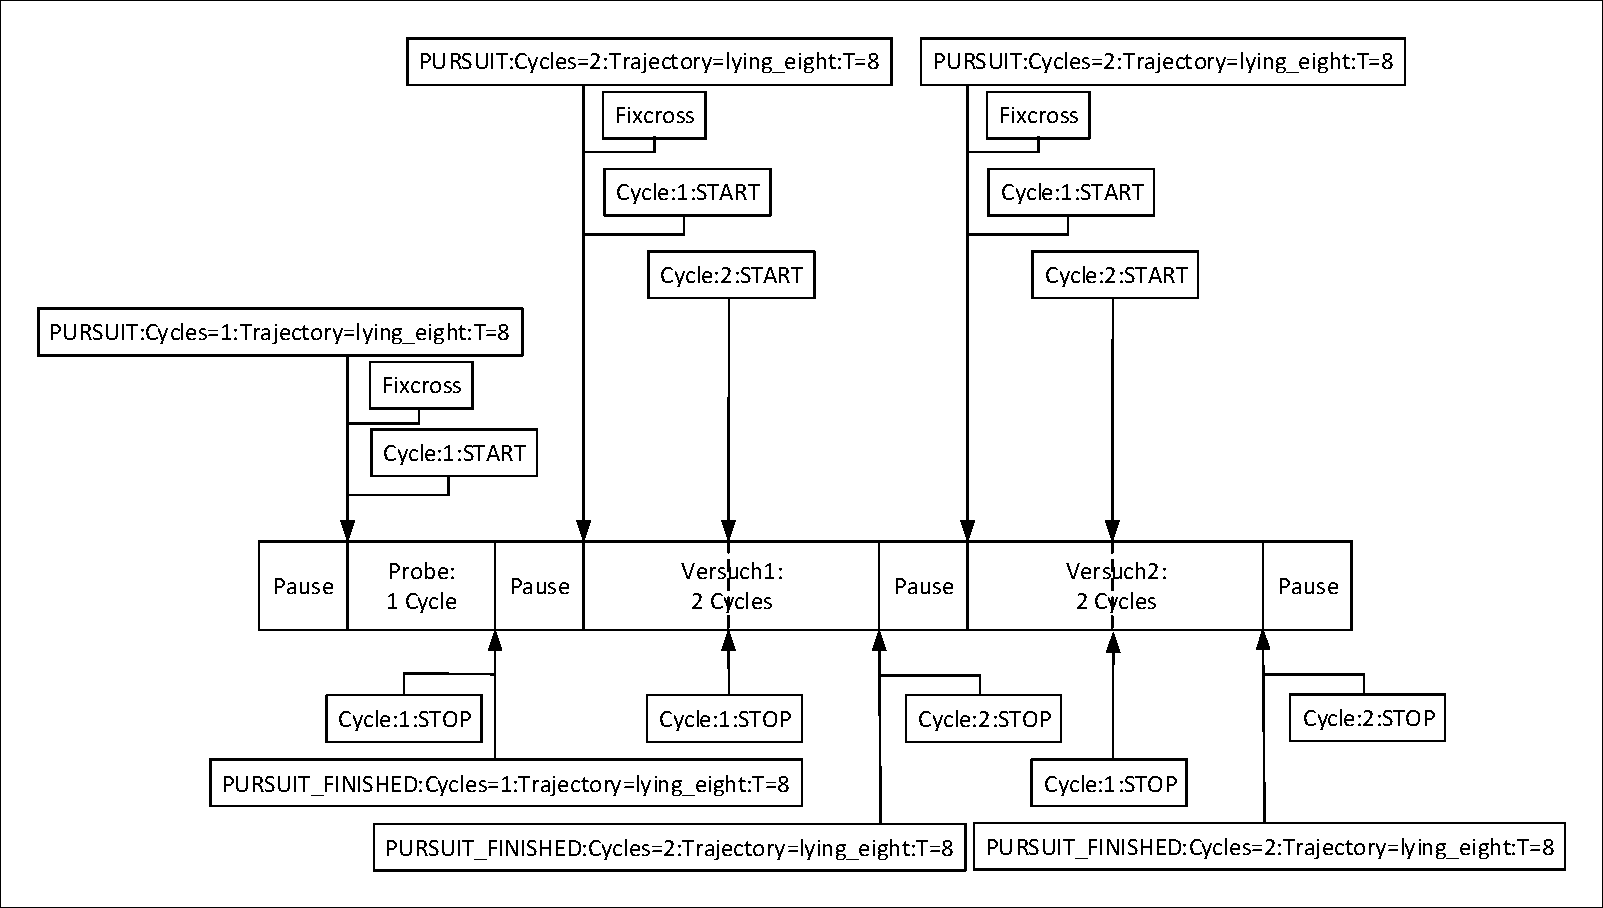
\includegraphics[width=15cm]{pics/Phasen-liegende-Acht.pdf}
		\par\end{centering}
	\caption{\label{fig:liegendeAcht}Phasen liegende Acht}
\end{figure}